\documentclass[tikz,border=2pt]{standalone}
\usepackage[T1]{fontenc}
\usepackage{lmodern}
\usetikzlibrary{arrows.meta,positioning,fit,backgrounds}
\begin{document}
\sffamily
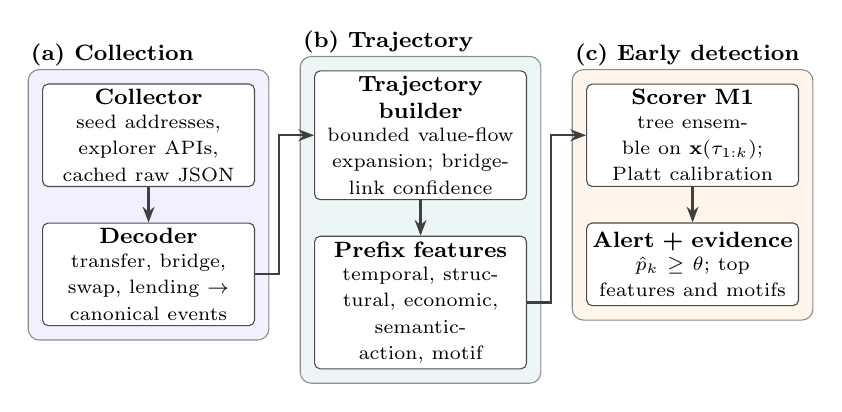
\begin{tikzpicture}[
  font=\footnotesize,
  stp/.style={draw=black!70, rounded corners=2pt, fill=white, text width=2.55cm, minimum height=1.05cm, align=center, inner sep=2pt},
  grp/.style={draw=black!45, rounded corners=4pt, inner sep=5pt},
  arr/.style={-{Stealth[length=2mm]}, thick, black!75},
  ttl/.style={font=\footnotesize\bfseries, anchor=south west, inner sep=1pt}
]
% Stage A: collection
\node[stp] (col) {\textbf{Collector}\\[-1pt]{\scriptsize seed addresses, explorer APIs, cached raw JSON}};
\node[stp, below=0.45cm of col] (dec) {\textbf{Decoder}\\[-1pt]{\scriptsize transfer, bridge, swap, lending $\to$ canonical events}};
% Stage B: processing
\node[stp, right=0.75cm of col] (traj) {\textbf{Trajectory builder}\\[-1pt]{\scriptsize bounded value-flow expansion; bridge-link confidence}};
\node[stp, below=0.45cm of traj] (feat) {\textbf{Prefix features}\\[-1pt]{\scriptsize temporal, structural, economic, semantic-action, motif}};
% Stage C: model
\node[stp, right=0.75cm of traj] (mod) {\textbf{Scorer M1}\\[-1pt]{\scriptsize tree ensemble on $\mathbf{x}(\tau_{1:k})$; Platt calibration}};
\node[stp, below=0.45cm of mod] (alert) {\textbf{Alert + evidence}\\[-1pt]{\scriptsize $\hat p_k\!\ge\!\theta$; top features and motifs}};
\begin{scope}[on background layer]
\node[grp, fill=blue!6, fit=(col)(dec), label={[ttl]north west:(a) Collection}] (ga) {};
\node[grp, fill=teal!7, fit=(traj)(feat), label={[ttl]north west:(b) Trajectory}] (gb) {};
\node[grp, fill=orange!8, fit=(mod)(alert), label={[ttl]north west:(c) Early detection}] (gc) {};
\end{scope}
\draw[arr] (col) -- (dec);
\draw[arr] (dec.east) -- ++(0.3,0) |- (traj.west);
\draw[arr] (traj) -- (feat);
\draw[arr] (feat.east) -- ++(0.3,0) |- (mod.west);
\draw[arr] (mod) -- (alert);
\end{tikzpicture}
\end{document}
